\documentclass[dvipsnames,mathserif]{beamer}
\setbeamertemplate{footline}[frame number]
\setbeamercolor{footline}{fg=black}
\setbeamerfont{footline}{series=\bfseries}
\usepackage{tikz}
\usepackage{xcolor}
\usepackage{graphicx, setspace, appendix, mathrsfs, amsmath, amsfonts,caption, mathtools}
\usepackage[english]{babel}
%\usetheme{Frankfurt}%1
\usetheme{Darmstadt}%1

% for RTL liste
\makeatletter
\newcommand{\RTListe}{\raggedleft\rightskip\leftm}
\newcommand{\leftm}{\@totalleftmargin}
\makeatother

% RTL frame title
\setbeamertemplate{frametitle}
{\vspace*{-1mm}
  \nointerlineskip
    \begin{beamercolorbox}[sep=0.3cm,ht=2.2em,wd=\paperwidth]{frametitle}
        \vbox{}\vskip-2ex%
        \strut\hskip1ex\insertframetitle\strut
        \vskip-0.8ex%
    \end{beamercolorbox}
}
% align subsection in toc
\makeatletter
\setbeamertemplate{subsection in toc}
{\leavevmode\rightskip=5ex%
  \llap{\raise0.1ex\beamer@usesphere{subsection number projected}{bigsphere}\kern1ex}%
  \inserttocsubsection\par%
}
\makeatother

% RTL triangle for itemize
\setbeamertemplate{itemize item}{\scriptsize\raise1.25pt\hbox{\donotcoloroutermaths$\blacktriangleleft$}} 

%\setbeamertemplate{itemize item}{\rule{4pt}{4pt}}

\defbeamertemplate{enumerate item}{square2}
{\LR{
    %
    \hbox{%
    \usebeamerfont*{item projected}%
    \usebeamercolor[bg]{item projected}%
    \vrule width2.25ex height1.85ex depth.4ex%
    \hskip-2.25ex%
    \hbox to2.25ex{%
      \hfil%
      {\color{fg}\insertenumlabel}%
      \hfil}%
  }%
}}

\setbeamertemplate{enumerate item}[square2]
\setbeamertemplate{navigation symbols}{}


\titlegraphic { 
\begin{tikzpicture}[overlay,remember picture, opacity=0.1,]
\node[] at (0, 2.9){
};\end{tikzpicture}}
\setbeamertemplate{caption}[numbered]
\begin{document}

\rightskip\rightmargin
\title{The role of information acquisition in matching markets: China's college admission mechanisms}
\author{Yao Luo}


\institute{Boston College}
\footnotesize{\date{\today }


\begin{frame}
\maketitle
\end{frame}


%\footnotesize \tableofcontents
%
\section{Motivation}
\begin{frame}{Motivation}
    \begin{itemize}
        \item Parallel admission mechanism (PA) - Direct serial dictatorship with length restriction of the rank-ordered list (ROL)\\
        \item Inner Mongolia dynamic admission mechanism (IM) - Sequential serial dictatorship + sequential moves by groups instead of individuals + time constraints\\
        \item Theoretically and experimentally, a sequential serial dictatorship mechanism leads to higher student welfare than a direct serial dictatorship mechanism. (Hakimov et all, 2023)

    \end{itemize}
\end{frame}
\begin{frame}{Motivation}
\begin{figure}[h!]
\centering
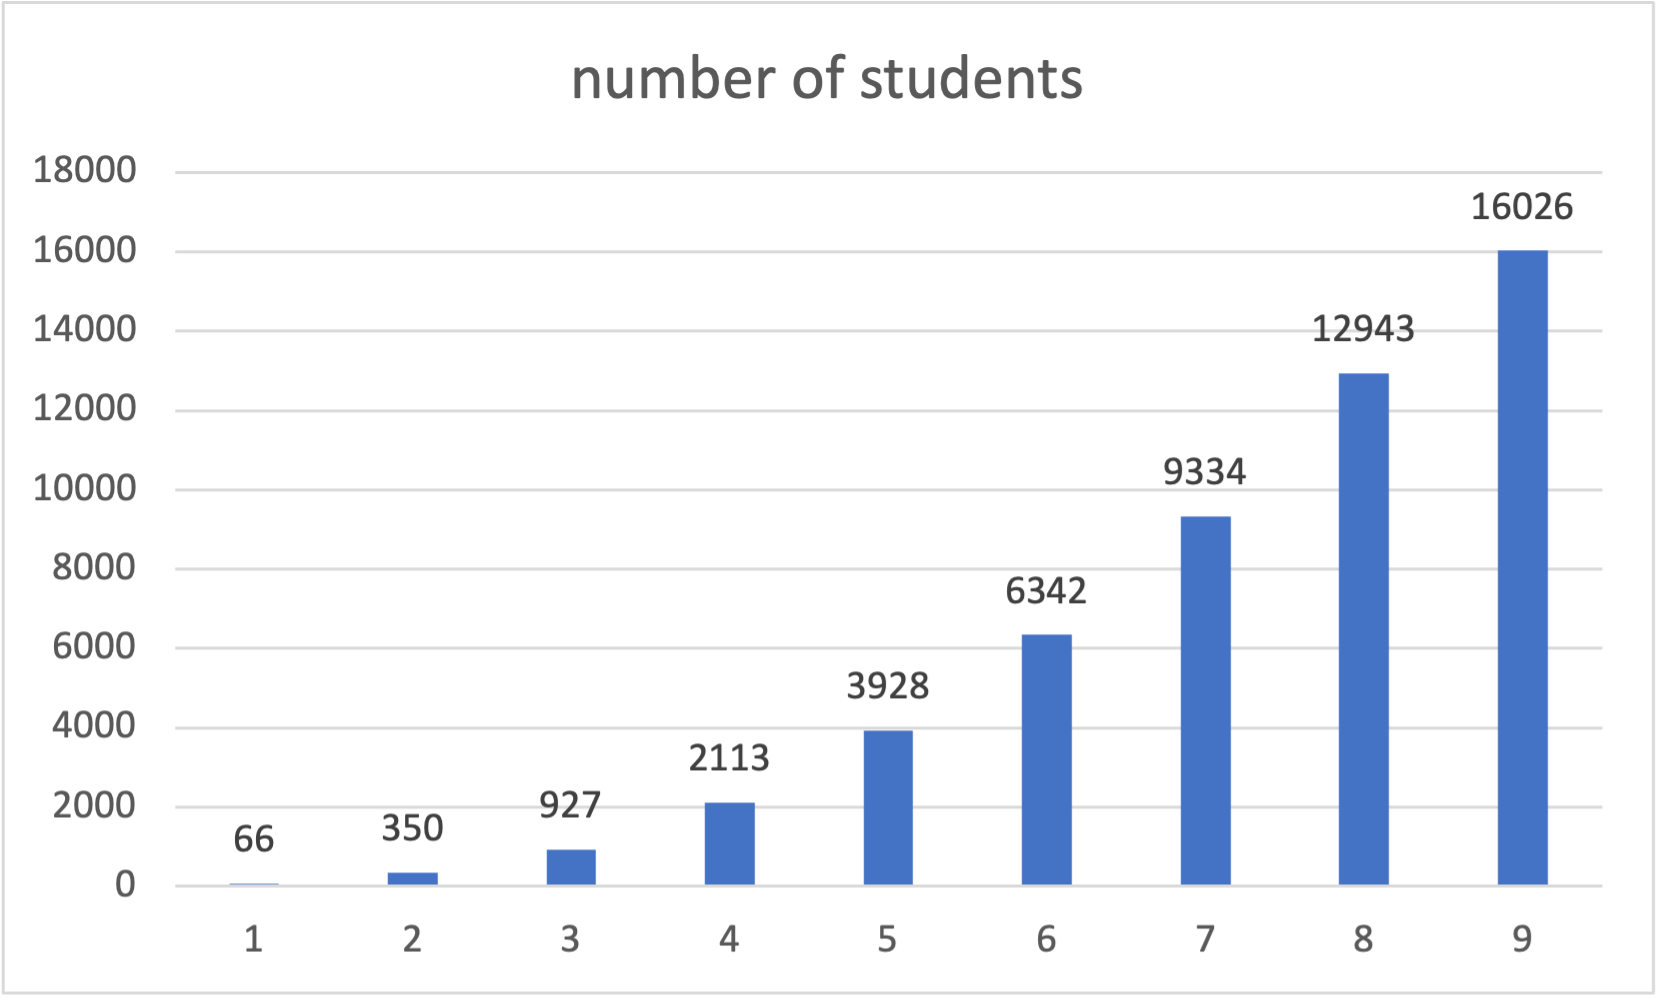
\includegraphics[width=0.8\textwidth]{1.png}
\end{figure}
\end{frame}

\begin{frame}{Motivation}
Theoretical results tell us:
\vspace{0.5cm}
    \begin{itemize}
        \item Traditional matching literature assume full information. But ... show that people need to conduct costly information acquisition to discover their preferences.\\
        \item Market designers should pay attention to information flows.\\
        \item Follow Azevedo and Loshno (2016) and Immorlica et al (2020), finding regret-free stable matching outcomes is equivalebt to finding market-clearing cutoffs.\\
        \item Imposibility stems from information deadlocks. Regret-free stable outcomes can not be achieved.
    \end{itemize}
\end{frame}
\begin{frame}{Motivation}
Real mechanism implementations:
\vspace{0.5cm}
    \begin{itemize}
        \item Achieve approximately regret-free stable outcomes by providing external historical data with respect to perturbed capacities: Australia\\
        \item In 2023 Australia has 62,846 applicants, while China has 12,910,000 applicants. \\
        \item Both PA and IM provides historical cutoff scores, but IM offers additional information regarding matching outcomes.\\
        \item In 2025 Inner Mongolia will give up IM and use PA. IM began in 2007. 
    \end{itemize}
\end{frame}




\section{Research question}
\begin{frame}{Research question}
    \begin{itemize}
    	\item First guess IM better than PA since IM provides additional information. Seems counterituitive.\\
    	\item Maybe the time constraints in IM (one hour per group) make the price discovery process too costly. Maybe information communication in IM is not effective. Maybe the additional information is too noisy and detriment students' welfare instead. Or maybe IM is indeed better than PA and the policy change is purely of political intention. 
        \item Are there better ways to communicate information to students to improve matching outcomes of IM? \\
    \end{itemize}
\end{frame}

\section{Contribution}
\begin{frame}{Contribution}
    \begin{itemize}
        \item Provide empirical and experimental results about comparisions of PA and IM mechanisms. \\
        \item Gong and Liang (2023) shows experimentally IM mechanism achieves similar stability as DA mechanism and similar efficiency as Bostom mechanism under incomplete information, when there is low correlation of preferences.\\
        \item Chen and Kesten (2019) shows experimentally DA mechanism is better than PA in terms of stability, but the setup assumes complete information.   
    \end{itemize}
\end{frame}


\section{A natural experiment}
\begin{frame}{A natural experiment}
	\begin{itemize}
		\item Data: students' exam score, rank and admission result.
        \item \[y_i = \alpha_0 + \alpha_1 X_i + \beta Y_{2025} + \varepsilon_i\]
        where $y_i$ is previliage index calculated by dividing the rank of the college (determined by cutoff scores) by the total number of colleges.\\
        $X_i$ includes students' gender, ethnicity, rank by exam scores being normalized to be within (0,1).\\
        \item Implicitly assumes higher-ranked students prefer more prestigious colleges. Only care about big names without considering majors. \\
        \item \[\rho = 1 -  \frac{6\Sigma_{i}^{N}d_i^2}{n(n^2-1)}\]
        Spearman's rank correlation coefficient.
    \end{itemize}
\end{frame}

\section{Experiment design}
\begin{frame}{Experiment design}
General setup:
    \begin{itemize}
        \item Students know their exam scores, ranks, each university's quotas and historical cutoffs. 
        \item 30 students competing for 15 seats in 10 colleges. Admission rate is 50\%.
        \item Preferences are private knowledge. Students need to pay search costs to acquire information about their own preferences.\\
    \end{itemize}
Variations:
	\begin{itemize}
		\item Dimension 1: The degree of correlation of preferences among students.\\
		\item Dimension 2: The cost of information acquisiton.
	\end{itemize}
\end{frame}

\begin{frame}{Experiment design}
Predictions:
    \begin{itemize}
        \item Hypothesis 1: Lower-ranked students gain more from IM compared to PA.\\
        \item Hypothesis 2: Lowest-ranked student in each group is worse off than under PA.\\ 
        \item Hypothesis 3: Given an extended time constraint, students may oversearch.\\
        \item Hypothesis 4: Smaller group size produces better matching outcomes.\\
        \item Hypothesis 5: Increasing the ROL in PA improves the matching outcomes.
    \end{itemize}
\end{frame}


\end{document}